\section{Weighted Finite State Automata (WFSA)}
\emph{Task} --- Determine whether a string is an element of a given language

{\color{lightgray}\hrule height 0.001mm}

\emph{Background} ---
\begin{itemize}
    \item String $s$
    \item Empty string $\varepsilon$
    \item Set of all strings given by Kleene closure $\Sigma^*$
    \item String language $L$, subset of $\Sigma^*$ 
\end{itemize}

\subsection*{(W)FSA | Finite State Automata (FSA)}
\emph{Formalization} --- 
\begin{itemize}
    \item $\mathcal{A}$ is a 5-tuple $(\Sigma, Q, I, F, \delta)$
    \begin{itemize}
        \item $\Sigma$ is an alphabet, consisting of letters $a,b,c,...$
        \item $Q$ is a finite set of states
        \item $I \subseteq Q$ is the set of initial states, usually only one
        \item $F \subseteq Q$ is the set of final or accepting states, can be multiple
        \item $\delta \subseteq Q \times (\Sigma \cup \{\varepsilon\}) \times Q$ resp. $q \xrightarrow{a \in \Sigma \cup \{\varepsilon\}} q'$ is a finite multiset of transitions from one state in $Q$ to another state in $Q$ via a symbol in $\Sigma$ 
    \end{itemize}
    \item Can be represented as a directed, possibly cyclical graph
    \item Sequentially reads individual symbols of an input string $s$ and transitions from state $q$ to state $q'$ upon reading a symbol $a$ iff $(q, a, q') \in \delta$
    \item If the automaton, after reading the last symbol of $s$, ends up in a state $q_f \in F$, the automaton \emph{accepts} the string
\end{itemize}

{\color{black}\hrule height 0.001mm}

\subsection*{(W)FSA | Weighted Finite State Automata (WFSA)}
\begin{itemize}
    \item Generalization of FSA, where transitions are weighted with a semiring: Unweighted FSA corresponds to WFSA weighted with Boolean semiring
    \item $\mathcal{A}$ is a 7-tuple $(\Sigma, Q, I, F, \delta, \lambda, \rho)$ over a semiring $\mathcal{W} = (\mathbb{K}, \oplus, \otimes, 0, 1)$ which, vs. FSA, defines:
    \begin{itemize}
        \item $I = \{q \in Q \mid \lambda(q) \neq 0\} \subseteq Q$
        \item $F = \{q \in Q \mid \rho(q) \neq 0\} \subseteq Q$ 
        \item $\delta \subseteq Q \times (\Sigma \cup \{\varepsilon\}) \times \mathbb{K} \times Q$ resp. $q \xrightarrow{a \in \Sigma \cup \{\varepsilon\} / w} q'$ is a finite multiset of weighted transitions from one state in $Q$ to another state in $Q$ via a symbol in $\Sigma$
        \item $\lambda : Q \to \mathbb{K}$ is an initial weighting function over $Q$, is $\overline{0}$ for non-initial states
        \item $\rho : Q \to \mathbb{K}$ is a final weighting function over $Q$, is $\overline{0}$ for non-final states
    \end{itemize}
\end{itemize}

{\color{black}\hrule height 0.001mm}

\subsection*{(W)FSA | (W)FSA Terminology}
\begin{itemize}
    \item \emph{Paths}:
    \begin{itemize}
        \item A path $\pi$ is an element of $\delta^*$ with consecutive transitions:
        $
        q_1 \xrightarrow{a_1/w_1} q_2,q_2 \xrightarrow{a_2/w_2} q_3, \cdots, q_{N-1} \xrightarrow{a_N/w_N} q_N
        $
        \item $\textrm{p}(\pi) = q_1$ is the beginning state of the path
        \item $\textrm{q}(\pi) = q_N$ is the ending state of the path
        \item \emph{Length} of path $|\pi|$ is the number of transitions
        \item \emph{Yield} of path $s(\pi)$ is the concatenation of symbols on the path
        \item Path sets: Denoted by capital $\Pi$
        \begin{itemize}
            \item $\Pi(\mathcal{A})$: Set of all paths in the automaton
            \item $\Pi(s)$: Set of all paths with yield $s$
            \item $\Pi(q)$: Set of all paths starting at $q$
            \item $\Pi(q, q')$: Set of all paths from $q$ to $q'$
            \item $\Pi(q, s, q')$: Set of all paths from $q$ to $q'$ with yield $s$
            \item $\Pi(\mathcal{Q}) = \bigcup_{q \in Q} \Pi(q)$
            \item $\Pi(\mathcal{Q}, \mathcal{Q}') = \bigcup_{q \in Q, q' \in Q'} \Pi(q, q')$
            \item $\Pi(\mathcal{Q}, s, \mathcal{Q}') = \bigcup_{q \in Q, q' \in Q'} \Pi(q,s,q')$
        \end{itemize}
        \item \emph{Inner path weight} $w_I(\pi)$ of a path $\pi = q_0 \xrightarrow{a_1/w_1} q_1 \cdots q_{N-1} \xrightarrow{a_N/w_N} q_N$:
        $
        w_I(\pi) = \bigotimes_{n=1}^N w_n
        $
        \item \emph{Path weight} $w(\pi)$ of a path:
        $
        w(\pi) = \lambda(\textrm{p}(\pi)) \otimes w_I(\pi) \otimes \rho(\textrm{q}(\pi))
        $
        \item A path is \emph{accepting resp. successful} iff $w(\pi) \neq 0$
    \end{itemize}

    \item \emph{Cycles}:
    \begin{itemize}
        \item A path is a cycle if starting and finishing states are the same
        \item A path contains a cycle if the same state appears multiple times
    \end{itemize}

    \item Transitions:
    \begin{itemize}
        \item Outgoing arcs from $q$: $E_\mathcal{A} (q) = \{a, t, w \mid (q, a, w, t) \in \delta\}$
        \item Incoming arcs to $q$: $E_\mathcal{A}^{-1} (q) = \{a, s, w \mid (s, w, a, q) \in \delta\}$
    \end{itemize}

    \item States:
    \begin{itemize}
        \item State $q$ is \emph{accessible} iff $q \in I$ or there exists a path whose weight is not 0 from $I$ to $q$
        \item State $q$ is \emph{co-accessible} iff $q \in F$ or there exists a path whose weight is not 0 from $q$ to $F$
        \item States that are either not accessible or not co-accessible are called \emph{useless}
    \end{itemize}

    \item (W)FSA is \emph{unambiguous} iff for every string $s$ there is at most one accepting path
\end{itemize}

{\color{black}\hrule height 0.001mm}

\subsection*{WFST | Weighted Finite State Transducers (WFST)}
\emph{Task} --- Transforms input string in a given language to output string in a given language, e.g. $\textrm{Muse} \to \mu ou \sigma \alpha$

{\color{lightgray}\hrule height 0.001mm}

\emph{Background} ---
\begin{itemize}
    \item $\boldsymbol{x}$: Input string
    \item $\boldsymbol{y}$: Transliteration of input string
\end{itemize}

{\color{lightgray}\hrule height 0.001mm}

\emph{Formalization} --- 
\begin{itemize}
    \item $\mathcal{T}$ is an 8-tuple $(\Sigma, \Omega, Q, I, F, \delta, \lambda, \rho)$ over a semiring $\mathcal{W} = (\mathbb{K}, \oplus, \otimes, 0, 1)$ which, vs. WFSA, defines:
    \begin{itemize}
        \item $\Sigma$ is the input alphabet 
        \item $\Omega$ is the output alphabet 
        \item $\delta \subseteq Q \times (\Sigma \cup \{\varepsilon\}) \times (\Omega \cup \{\varepsilon\}) \times \mathbb{K} \times Q$ resp. $q \xrightarrow{a \in \Sigma \cup \{\varepsilon\} : b \in \Omega \cup \{\varepsilon\} / w} q'$ is a finite multiset of weighted transitions from one state in $Q$ to another state in $Q$ via a symbol in $\Sigma$ and in $\Omega$
    \end{itemize}
\end{itemize}

{\color{black}\hrule height 0.001mm}

\subsection*{WFST | Compositions}
\begin{itemize}
    \item Operation to combine two or more WFSTs
    \item $\mathcal{T}_1 \circ \mathcal{T}_2$ is the composition of $\mathcal{T}_1 = (\Sigma, \Omega, Q_1, I_1, F_1, \delta_1, \lambda_1, \rho_1)$ and $\mathcal{T}_2 = (\Omega, \Gamma, Q_2, I_2, F_2, \delta_2, \lambda_2, \rho_2)$ and is given by:
    $
    \mathcal{T} = (\Sigma, \Gamma, Q, I, F, \delta, \lambda, \rho)
    $
    such that:
    $
    \mathcal{T}(x, y) = \bigoplus_{z \in \Omega^*} \mathcal{T}_1(x, z) \otimes \mathcal{T}_2(z, y)
    $ where $\mathcal{T}(i,j)$ is the weight assigned by the transducer to a mapping from an input string $i$ to an output string $j$
    \item Naive algorithm to compute composition:
    \begin{enumerate}
        \item $\mathcal{T} \gets (\Sigma, \Omega, Q, I, F, \delta, \lambda, \rho)$ to create a new WFST
        \item Create initial state $(q_1^i, q_2^i) \in I_1 \times I_2$ and final state $(q_1^f, q_2^f) \in F_1 \times F_2$
        \item For $q_1, q_2 \in Q_1 \times Q_2$:\\
        For
        $
        (q_1 \xrightarrow{a:b/w_1} q_1'), (q_2 \xrightarrow{c:d/w_2} q_2') \in  E_{\mathcal{T}_1}(q_1) \times E_{\mathcal{T}_2}(q_2):
        $\\
        If 
        \begin{itemize}
            \item $b=c$
            \item $(q_1, q_2)$ and $(q_1', q_2')$ are both accessible (reachable from $(q_1^i, q_2^i)$) in the composed transducer
            \item $(q_1, q_2)$ and $(q_1', q_2')$ are both co-accessible (can reach $(q_1^f, q_2^f)$) in the composed transducer
        \end{itemize}
        \begin{itemize}
            \item Add states $(q_1, q_2)$, $(q_1', q_2')$ to $\mathcal{T}$ if they have not yet been added
            \item Add arc $(q_1, q_2) \xrightarrow{a:d/w_1 \otimes w_2} (q_1', q_2')$ to $\mathcal{T}$
        \end{itemize}
        \item For $(q_1^i, q_2^i) \in I_1 \times I_2$: $
        \lambda_\mathcal{T} = \lambda_1(q_1^i) \otimes \lambda_2(q_2^i)
        $
        \item For $(q_1^f, q_2^f) \in F_1 \times F_2$: $
        \rho_\mathcal{T} = \rho_1(q_1^f) \otimes \rho_2(q_2^f)
        $
        \item Return $\mathcal{T}$
    \end{enumerate}
    \item Challenge: Runs through many useless states, has runtime complexity $\mathcal{O}(|Q_1||Q_2|)$
    \item Solution: \emph{Accessible algorithm}
    \item \emph{Accessible algorithm}:
    \begin{itemize}
        \item Intuition: Construct all possible pairs of initial states and then expand outwards (depth-first search), adding accessible states
        \item Note: Produced states may still be non-co-accessible
        \begin{enumerate}
            \item $\textrm{stack} \gets [(q_1, q_2) \mid q_1 \in I_1, \, q_2 \in I_2]$ (ordered list, allows duplicates)\\
            $\textrm{visited} \gets \{(q_1, q_2) \mid q_1 \in I_1, \, q_2 \in I_2\}$ (unordered set, does not allow duplicates)
            \item $\mathcal{T} \gets (\Sigma, \Omega, Q, I, F, \delta, \lambda, \rho)$ to create a new WFST
            \item While $|\textrm{stack}| > 0$:
            \begin{enumerate}
                \item $q_1, q_2 \gets \textrm{stack.pop()}$
                \item For:
                $
                (q_1 \xrightarrow{a:b/w_1} q_1'), \quad (q_2 \xrightarrow{c:d/w_2} q_2') \in E_{\mathcal{T}_1}(q_1) \times E_{\mathcal{T}_2}(q_2)$:\\
                If $b=c$:
                \begin{enumerate}
                    \item Add states $(q_1, q_2)$, $(q_1', q_2')$ to $\mathcal{T}$ if they have not yet been added
                    \item Add arc $(q_1, q_2) \xrightarrow{a:d/w_1 \otimes w_2} (q_1', q_2')$ to $\mathcal{T}$
                    \item If $(q_1', q_2')$ not in visited: Push $(q_1', q_2')$ to stack and visited
                \end{enumerate}
            \end{enumerate}
            \item For $(q_1^i, q_2^i) \in I_1 \times I_2$: $
            \lambda_\mathcal{T} = \lambda_1(q_1^i) \otimes \lambda_2(q_2^i)
            $
            \item For $(q_1^f, q_2^f) \in F_1 \times F_2$: $
            \rho_\mathcal{T} = \rho_1(q_1^f) \otimes \rho_2(q_2^f)
            $
        \end{enumerate}
    \end{itemize}
\end{itemize}

{\color{black}\hrule height 0.001mm}

\subsection*{(W)FSA | Pathsum and Lehmann's algorithm}
\emph{Pathsum} ---
\begin{itemize}
    \item \emph{Pathsum} of $\mathcal{A}$:
    $
    Z(\mathcal{A}) = \bigoplus_{\pi \in \Pi(\mathcal{A})} w(\pi)
    $
    \item Pathsum in different semirings:
    \begin{itemize}
        \item Pathsum is equal to the shortest path weight in the tropical semiring where $\otimes = +$ and $\oplus = \min$
        \item Pathsum is equal to the sum of all paths in the inside semiring where $\otimes = \times$ and $\oplus = +$
        \item In a $\overline{0}$-closed semiring:
        \begin{itemize}
            \item Pathsum depends only on paths of length $N-1$, since paths of length $\geq N$ contain cycles, but cycles do not improve the pathsum in $\overline{0}$-closed semirings, since $\overline{1} \oplus a = \overline{1}$
            \item Then, in Lehmann's algorithm, $\boldsymbol{R}* = \bigoplus_{n=0}^{N-1} \boldsymbol{R}^{\otimes n}$
            \item This has time complexity of $O((N-1) \times (N^3 + N^2))$, since we need to multiply over matrix of size $N \times N$ ($O(N^3)$), sum  over matrix of size $N \times N$ ($O(N^2)$) for $N-1$ iterations
            \item For idempotent semirings, where we can leverage binary decomposition, has time complexity of $O(\log_2(N-1) \times N^3 + (N-1) \times N^2)$, since we can pre-compute the $\log_2(N-1)$ required powers $\boldsymbol{R}^{2^k}$ for matrix multiplication
        \end{itemize}
    \end{itemize}
\end{itemize}
Pathsum in acyclic WFSA:
\begin{itemize}
    \item In acyclic WFSA, the number of accepting paths is finite, thus $Z(\mathcal{A})$ is finite
    \item To compute pathsum $Z(\mathcal{A})$, we need a topological sort of the nodes (starts with initial state and progresses towards final state)
    \item Backward algorithm:
    \begin{itemize}
        \item Computes $Z(\mathcal{A})$
        \begin{enumerate}
            \item For $q \in \textrm{Rev-Top}(\mathcal{A})$ (starts with final state and progresses towards initial state):
            \begin{enumerate}
                \item If $q \in F$: $
                \beta(q) = \rho(q)
                $
                \item Else: $
                \beta(q) = \bigoplus_{q \xrightarrow{a/w} q'} \quad w \otimes \beta(q')
                $
            \end{enumerate}
            \item Return:
            $
            \bigoplus_{q^i \in I} \lambda(q^i) \otimes \beta(q^i)
            $
        \end{enumerate}
        \item Runs in $\mathcal{O}(|\delta|)$ time and $\mathcal{O}(|Q|)$ space
        \item Could alternatively also be computed as forward algorithm:
        \begin{enumerate}
            \item For $q \in \textrm{Top}(\mathcal{A})$:
            \begin{enumerate}
                \item If $q \in I$: $
                \alpha(q) = \lambda(q)
                $
                \item Else: $
                \alpha(q) = \bigoplus_{q' \xrightarrow{a/w} q} \quad w \otimes \alpha(q')
                $
            \end{enumerate}
            \item Return:
            $
            \bigoplus_{q^f \in F} \rho(q^f) \otimes \beta(q^f)
            $
        \end{enumerate}
    \end{itemize}
\end{itemize}
Pathsum in cyclical WFSA:
\begin{itemize}
    \item In cyclical WFSA, the number of accepting paths is infinite, thus $Z(\mathcal{A})$ is infinite
    \item Lehmann's algorithm can nonetheless calculate $Z(\mathcal{A})$
    \item To use this algorithm, we need to represent WFSA as a matrix:
        \begin{itemize}
            \item Define $|\Sigma|$ \emph{adjacency matrices}, one for each transition symbol $a \in \Sigma$: $\boldsymbol{W}^{(a)} \in \mathbb{R}^{(|Q| \times |Q|)}$: Contains the from-states $q_n$ in the rows and the to-states $q_m$ in the columns, entries are given by the weight $w$ for the transition $q_n \xrightarrow{a /w}  q_m$ if it exists, otherwise $\overline{0}$
            \item Since in the pathsum all paths are summed, we can collapse all transitions from $q_n$ to $q_m$ into a single transition without a label, whose weight is the $\oplus$-sum of all original transitions:
            $
            \boldsymbol{W} = \bigoplus_{a \in \Sigma \cup \{\varepsilon\}} \boldsymbol{W}^{(a)}
            $
            \item Pathsum for paths between node $q_n$ to node $q_m$ of length exactly $l$ can be calculated via matrix multiplication of the adjacency matrix: $\boldsymbol{W}^l = \boldsymbol{W} \otimes \boldsymbol{W} \otimes ...$\\
            Proof: Matrix multiplication given by $(\boldsymbol{W} \otimes \boldsymbol{W})_{nm} = \bigoplus_{i=1}^{|Q|} \boldsymbol{W}_{ni} \otimes \boldsymbol{W}_{im}$. Thus, we compute the $\otimes$-product of the weights along any given path between $q_n$ and $q_m$. Then, we sum the computed weights across all paths between $q_n$ and $q_m$
        \end{itemize}
\end{itemize}
\emph{Lehmann's algorithm}:
\begin{itemize}
    \item Computes $Z(\mathcal{A})$ by computing Kleene closure of matrix $\boldsymbol{R}$ over closed semiring
    \item Algorithm: Computing $Z(\mathcal{A})$
    \begin{enumerate}
        \item Lehmann algorithm computes $\boldsymbol{R}$ with $|Q|^2$ entries. Each entry represents the $\oplus$-sum of the weights over the path between two nodes $q_i, q_k$:
        $
        \boldsymbol{R}_{ik} = \bigoplus_{\pi \in \Pi(q_i, q_k)} w_I(\pi)
        $
        where cyclical terms (either single nodes, or node combinations) are denoted with $*$
        \item From $\boldsymbol{R}$, we can compute $Z(\mathcal{A})$:
        $
        Z(\mathcal{A}) = \bigoplus_{i,k=1}^{|Q|} \lambda(q_i) \otimes \boldsymbol{R}_{ik} \otimes \rho(q_k)
        $ where only pairs $(i,k)$ are retained where $i$ is initial state and $k$ is final state, since for all other pairs either $\lambda(q_i) = \overline{0}$ or $\rho(q_k) = \overline{0}$
    \end{enumerate}
    \item Algorithm for step 1: Computing $\boldsymbol{R}$:
    \begin{enumerate}
        \item $\boldsymbol{R}^{(0)} \gets \boldsymbol{W}$
        \item For $j \gets 1$ up to $|Q|$:\\
        For $i \gets 1$ up to $|Q|$:\\
        For $k \gets 1$ up to $|Q|$:\\
        $
        \boldsymbol{R}_{ik}^{\leq j} \gets \boldsymbol{R}_{ik}^{\leq j-1} \oplus \big(\boldsymbol{R}_{ij}^{\leq j-1} \otimes (\boldsymbol{R}_{jj}^{\leq j-1})^* \otimes \boldsymbol{R}_{jk}^{\leq j-1}\big)
        $
        \item Return:
        $
        \boldsymbol{I} \bigoplus \boldsymbol{R}^{(|Q|)}
        $ where $\boldsymbol{I}$ is the matrix with $\overline{1}$ on the diagonal and $\overline{0}$ everywhere else
    \end{enumerate}
    \item Intuition for step 1: Computing $\boldsymbol{R}$:
    \begin{itemize}
        \item 1) For paths that do not pass through intermediary nodes (i.e. for direct connections):
        $
        R^{\leq 0} = \boldsymbol{W}
        $ 
        \item 2) For paths that do pass through intermediary nodes: Let $\boldsymbol{\Pi}^{\leq j}(q_i, q_k)$ be paths between $q_i$ and $q_k$ that do not cross nodes with indices $> j$ and $\boldsymbol{R}_{ik}^{\leq j}$ be the pathsum for these paths
        \item We can partition the paths in $\boldsymbol{\Pi}^{\leq j}(q_i, q_k)$ into two subsets: Paths that do not cross $j$ and paths that do
        \item $\Rightarrow$ For paths that do not cross $j$: 
        \begin{itemize}
            \item $
            \pi \in \Pi^{\leq j-1}(q_i, q_k)
            $
            \item In that case, the pathsum is:
            $
            \boldsymbol{R}_{ik}^{\leq j-1}
            $
        \end{itemize}
        \item $\Rightarrow$ For paths that do cross $j$: 
        \begin{itemize}
            \item $\pi$ can be decomposed into cycle that starts and ends in $j$, part before cycle, and part after cycle: $
            \pi_{ij} \pi_{jj} \pi_{jk}
            $
            \item In that case, we can also decompose the pathsum into partial pathsums:
            $
            \boldsymbol{R}_{ij}^{\leq j-1} \otimes (\boldsymbol{R}_{jj}^{\leq j-1 })^* \otimes \boldsymbol{R}_{jk}^{\leq j-1}
            $
        \end{itemize}
        \item $\Rightarrow$ Combining these subsets, we get $
        \boldsymbol{R}_{ik}^{\leq j} \to \boldsymbol{R}_{ik}^{\leq j-1} \oplus \boldsymbol{R}_{ij}^{\leq j-1} \otimes (\boldsymbol{R}_{jj}^{\leq j-1 })^* \otimes \boldsymbol{R}_{jk}^{\leq j-1}
        $
        \item Clearly $\boldsymbol{R}_{ik}^{\leq |Q|} = \boldsymbol{R}_{ik}$
        \item This defines a natural procedure to build up the pathsum from the partial pathsums
    \end{itemize}
    \item Runs in $\mathcal{O}(|Q|^3)$ time
    \item Lehmann algorithm encompasses Floyd-Warshall algorithm and Gauss-Jordan algorithm
\end{itemize}

{\color{black}\hrule height 0.001mm}

\subsection*{Transliteration}
\emph{Motivation for using WFSAs resp. WFSTs} ---
Why can't we use a CRF?
\begin{itemize}
    \item In CRFs, we can only align sequences of the same length, e.g., $|\boldsymbol{x}| = |\boldsymbol{y}|$
    \item In WFSTs resp. WFSAs, we can align sequences of different lengths
\end{itemize}

{\color{lightgray}\hrule height 0.001mm}

\emph{Aim and approach} ---
Aim: Compute log-likelihood $p(\boldsymbol{y}|\boldsymbol{x}) = \frac{\exp(\textrm{score}(\boldsymbol{x},\boldsymbol{y}))}{Z}$ where $\textrm{score}(\boldsymbol{x}, \boldsymbol{y})$ is the pathsum $\log \sum_{\pi \in \Pi(\boldsymbol{y})} w(\pi)$\\
Approach:
\begin{itemize}
    \item We encode source sequence $\boldsymbol{x} \in \Sigma^*$ as WFST $\mathcal{T}_x$: This prepares $\boldsymbol{x}$ for alignment 
    \item We encode target sequence $\boldsymbol{y} \in \Omega^*$ as WFST $\mathcal{T}_y$: This prepares $\boldsymbol{y}$ for alignment
    \item We need a WFST $\mathcal{T}$ that maps string over $\Sigma$ to string over $\Omega$: Each path in $\mathcal{T}$ represents one alignment of some string in $\Sigma^*$ to some string in some string in $\Omega^*$
    \item We can generate the composition $\mathcal{T}_x \circ \mathcal{T}$: Each path in $\mathcal{T}_x \circ \mathcal{T}$ represents one alignment of $\boldsymbol{x}$ to some string in $\Omega^*$
    \item We can generate the composition $\mathcal{T}_x \circ \mathcal{T} \circ \mathcal{T}_y$: Each path in $\mathcal{T}_x \circ \mathcal{T} \circ \mathcal{T}_y$ represents one alignment of $\boldsymbol{x}$ to $\boldsymbol{y}$
    \item $p(\boldsymbol{y} \mid \boldsymbol{x})$ is then given by the probability of all paths in $\mathcal{T}_x \circ \mathcal{T}$ that align $\boldsymbol{x}$ to $\boldsymbol{y}$: $= \frac{\textrm{pathsum of } \mathcal{T}_x \circ \mathcal{T} \circ \mathcal{T}_y}{\textrm{pathsum of } \mathcal{T}_x \circ \mathcal{T}}$
    \item Training: To compute $p(\boldsymbol{y} \mid \boldsymbol{x})$, we can use Lehmann's algorithm with the log-sum-exp semiring
    \item Inference: To compute highest scoring $\boldsymbol{y}$ of composition $\mathcal{T}_x \circ \mathcal{T}$, we can use e.g. Dijkstra's algorithm or Floyd-Warshall algorithm with the arctic semiring and backpointers
    \item If we condition on $\boldsymbol{x}$ in WFST $\mathcal{T}_x \circ \mathcal{T}$, this WFST becomes a WFSA
\end{itemize}

{\color{lightgray}\hrule height 0.001mm}

\emph{Training: Lehmann's Algorithm} ---
\begin{itemize}
    \item $\mathcal{A}_x$ is the WFSA with:
    \begin{itemize}
        \item $\boldsymbol{\lambda}$ is a vector of start weights for starting states: $\lambda_n = \lambda(q_n)$
        \item $\boldsymbol{\rho}$ is a vector of end weights for ending states: $\rho_n = \rho(q_n)$
        \item Set of adjacency matrices, one for each output symbol: $\boldsymbol{W}^{(\omega)}$ for any $\omega \in \Omega \cup \{\varepsilon\}$:
        $
        \boldsymbol{W}_{nm}^{(\omega)}$ is the weight for $q_n \xrightarrow{\omega} q_m
        $
        \item $\boldsymbol{W}^{(\omega)}$ can be collapsed into a single matrix:
        $
        \boldsymbol{W} = \sum_{\omega \in \Omega \cup \{\varepsilon\}} \boldsymbol{W}^{(\omega)}
        $
    \end{itemize}
\end{itemize}
Computation of $Z$:
\begin{itemize}
    \item $Z$ is given by:
    $
    Z(\boldsymbol{x}) = \sum_{\boldsymbol{y}' \in \Omega^*} \exp(\textrm{score}(\boldsymbol{x}, \boldsymbol{y}'))
    $\\
    $
    = \sum_{\boldsymbol{y}' \in \Omega^*} \exp \Big( \log \sum_{\pi \in \Pi(\boldsymbol{y}')} w(\pi) \Big)
    $\\
    $
    = \sum_{\boldsymbol{y}' \in \Sigma^*} \sum_{\pi \in \Pi(\boldsymbol{y}')} \lambda(\textrm{p}(\pi)) \otimes w_I(\pi) \otimes \rho(\textrm{q}(\pi))
    $\\
    $
    = \sum_{\boldsymbol{y}' \in \Sigma^*} \sum_{\pi \in \Pi(\boldsymbol{y}')} \lambda(\textrm{p}(\pi)) \otimes \prod_{n=1}^{| \pi |} w_n(\pi) \otimes \rho(\textrm{q}(\pi))
    $ which is the pathsum\\
    $
    = \sum_{q_n, q_m \in Q} \Big( \sum_{\pi \in \Pi(q_n, q_m)} w(\pi) \Big)
    $\\
    $
    = \sum_{q_n, q_m \in Q} \sum_{\pi \in \Pi(q_n, q_m)} \lambda(\textrm{p}(\pi)) \otimes w_I(\pi) \otimes \rho(\textrm{q}(\pi))
    $\\
    $
    = \sum_{q_n, q_m \in Q} \sum_{\pi \in \Pi(q_n, q_m)} \lambda(q_n) \otimes w_I(\pi) \otimes \rho(q_m)
    $\\
    $
    = \sum_{q_n, q_m \in Q} \lambda(q_n) \otimes (\sum_{\pi \in \Pi(q_n, q_m)} w_I(\pi)) \otimes \rho(q_m)
    $\\
    $
    = \sum_{q_n, q_m \in Q} \lambda(q_n) \otimes (\boldsymbol{W}^*)_{nm} \otimes \rho(q_m)
    $\\
    $
    = \boldsymbol{\lambda}^\intercal \boldsymbol{W}^* \boldsymbol{\rho}
    $ where $\boldsymbol{W}^*$ can be computed via Lehmann's algorithm
    \item In this way, we can compute log likelihood for a training instance 
    \item To go from a single training instance to the entire training dataset: $\sum_{n=1}^N \log p(\boldsymbol{y}^{(n)} \mid \boldsymbol{x}^{(n)}) = \sum_{n=1}^N \Big[ \textrm{score}_\theta(\boldsymbol{y}^{(n)}, \boldsymbol{x}^{(n)}) - \log Z_\theta(\boldsymbol{x}^{(n)}) \Big]$
\end{itemize}

{\color{lightgray}\hrule height 0.001mm}

\emph{Inference: Floyd-Warshall algorithm} ---
\begin{itemize}
    \item Aim: Find shortest distances between all pairs of nodes in a graph, where the weights of the edges in the path are additive
    \item Corresponds to Lehmann algorithm weighted over the tropical semiring
    \item Requirement: No negative cycles in the graph, since if there were negative cycles, we could always loop over the cycle to lower the pathsum
    \item Based on that requirement, we can drop $(\boldsymbol{R}_{jj}^{\leq j-1 })^*$ in Lehmann algorithm
\end{itemize}

{\color{black}\hrule height 0.001mm}

\subsection*{Lehmann's applications | Gauss-Jordan algorithm}
\begin{itemize}
    \item Aim: For matrix $\boldsymbol{M}^{D \times D}$, find $\boldsymbol{M}^{-1}$
    \item We know that, for matrix $\boldsymbol{M}$ Lehmann's algorithm computes $\boldsymbol{M}^*$
    \item We know that $\boldsymbol{M}^* = (\boldsymbol{I}-\boldsymbol{M})^{-1}$\\
    Proof:
    \begin{itemize}
        \item $
        \mathbf{M}^* = \mathbf{I} + \mathbf{M} \mathbf{M}^*
        $
        \item $
        \mathbf{M}^* - \mathbf{M} \mathbf{M}^* = \mathbf{I}
        $
        \item $
        \mathbf{M}^* (\mathbf{I} - \mathbf{M}) = \mathbf{I}
        $
        \item $
        \mathbf{M}^* = (\mathbf{I} - \mathbf{M})^{-1}
        $
    \end{itemize}
    \item Conversely, $(\boldsymbol{I}-\boldsymbol{M})^* = \boldsymbol{M}^{-1}$\\
    Proof:
    \begin{itemize}
        \item $(\mathbf{I} - \mathbf{M})^* = \mathbf{I} + (\mathbf{I} - \mathbf{M})(\mathbf{I} - \mathbf{M})^*$
        \item $(\mathbf{I} - \mathbf{M})^* - (\mathbf{I} - \mathbf{M})(\mathbf{I} - \mathbf{M})^* = \mathbf{I}$
        \item $(\mathbf{I} - \mathbf{M})^* (\mathbf{I} - (\mathbf{I} - \mathbf{M})) = \mathbf{I}$
        \item $(\mathbf{I} - \mathbf{M})^* = \mathbf{M}^{-1}$
    \end{itemize}
    \item Thus, we can get $\mathbf{M}^{-1}$ by running Lehmann algorithm on $(\mathbf{I} - \mathbf{M})$ weighted over the inside field (instead of semiring, since a field gives us subtraction and division)
\end{itemize}

{\color{black}\hrule height 0.001mm}

\subsection*{(W)FSA applications | N-gram, CRF, HMM}
\emph{N-gram models} --- 
\begin{itemize}
    \item Let $\boldsymbol{y} = (y_1, \ldots, y_L)$ be a string with $y_1 = \textrm{BOS}$, $y_L = \textrm{EOS}$
    \item Let N-gram be of order $N$
    \item We want to model 
    $
    p(y_n \mid y_{n-N+1}, \ldots, y_{n-1})
    $    
    \item If we represent this with WFSA:
    \begin{itemize}
        \item $\Sigma = V \cup \{\langle \textrm{BOS} \rangle, \langle\textrm{EOS} \rangle\}$
        \item States:
        \begin{itemize}
            \item Represent all N-grams
            \item $Q = \bigcup_{n=0}^N \{ \{\langle \textrm{BOS} \rangle\}^{N-n} \times V^{n-1} \times (V \cup \{\langle \textrm{EOS} \rangle\}) \}$\\
            E.g.: If $V = \{ \textrm{foo, bar} \}$:\\
            For bi-gram, we have the states $\textrm{BOS}, \textrm{foo}, \textrm{bar}, \textrm{EOS}$\\
            For tri-gram, we have the states $\textrm{BOS}\textrm{BOS}$, $ \textrm{BOS}\textrm{foo}$, $ \textrm{BOS}\textrm{bar}$, $ \textrm{foo}\textrm{foo}$, $ \textrm{bar}\textrm{bar}$, $ \textrm{foo}\textrm{bar}$, $ \textrm{bar}\textrm{foo}$, $ \textrm{foo}\textrm{EOS}$, $
            \textrm{bar}\textrm{EOS}$, $
            \textrm{BOS}\textrm{EOS}$
            \item $q_{ij...}$ represents the state where the N-gram's most recent word $y_n  = i$, the second-most recent word $y_{n-1}  = j$, etc.
        \end{itemize}
        \item $I = \{\langle \textrm{BOS}, \ldots, \textrm{BOS} \rangle\}$ ($N$ times) is a subset of $Q$ at $n=0$
        \item $F = Q$
        \item Transitions:
        \begin{itemize}
            \item $\delta = \big\{ (y_{-N} \ldots y_{-1}, y_0, p(y_0 \mid y_{-N+1}, \ldots, y_{-1}), y_{-N+1} \ldots y_0 )$\\
            for $(y_{-N+1} \ldots y_{-1}) \in \bigcup_{n=0}^{N-1} \{ \langle \textrm{BOS} \rangle \}^{N-1-n} \times V^n  \big\}$
            \item $
            \delta(q_{ij...}, y_n, 1, q_{ki...}) = 
            \begin{cases} 
                \log(p(y_n = k \mid y_{n-1}  = i, y_{n-2}  = j, \ldots, y_{n-N+1} = \ldots))\\
                \quad \textrm{if } y_n=k \\
                -\infty \textrm{ otherwise}
            \end{cases}
            $
            \item Transitions are only defined if N-gram order $\geq 2$
            \item Only transitions between N-grams which can follow each other are allowed and receive weights $> \overline{0}$
            \item The weight represents the probability of $
            p(y_n \mid y_{n-N+1}, \ldots, y_{n-1})
            $
        \end{itemize}
        \item Initial state:
        \begin{itemize}
            \item $\lambda = \langle \textrm{BOS} \rangle \ldots \langle \textrm{BOS} \rangle \to \overline{1}$ ($N$ times) i.e. state corresponding to full padding of $\textrm{BOS}$ receives weight $\overline{1}$
            \item $\lambda(q_{ij...}) = \log(p(y_n = i \mid y_{n-1}  = \textrm{BOS}, y_{n-2}  = \textrm{BOS}, \ldots, y_{n-N+1} = \textrm{BOS}))$
        \end{itemize}
        \item Final state:
        \begin{itemize}
            \item $\rho = y_{n-N+1} \ldots y_1 \ \langle \textrm{EOS} \rangle \to \overline{1}$ i.e. state ending with $\textrm{EOS}$ receives weight $\overline{1}$
            \item $
            \rho(q_{ij...}) = \log(p(y_n = \textrm{EOS} \mid y_{n-1}  = i, y_{n-2}  = j, \ldots, y_{n-N+1} = \ldots))$
        \end{itemize}
    \end{itemize}
    \item We can compute $p(\boldsymbol{y}) = \lambda(q_I) + \sum_{n=1}^{L} \delta(q_{y_{n-N}, ..., y_{n-1}}, y_n, q_{y_{n-N+1}, ..., y_{n}}) + \rho(q_F)$
    \item For a vocabulary $V$, there are $x + |V|^{N-1} + z$ states:
    \begin{itemize}
        \item $|V|^{N-1}$ intermediate states with full N-gram history
        \item $x = \begin{cases} 
            |V|^{N-2} & \textrm{for N-grams with } N \geq 2 \\ 
            0 & \textrm{for unigrams} 
        \end{cases}$ start states with $\textrm{BOS}$ padding
        \item $z = \begin{cases} 
            1 & \textrm{for N-grams with } N \geq 2 \\ 
            0 & \textrm{for unigrams} 
        \end{cases}$ end states
    \end{itemize}
\end{itemize}

{\color{lightgray}\hrule height 0.001mm}

\emph{CRFs} --- 
\begin{itemize}
    \item Let $|\boldsymbol{x}| = L$ and $|\boldsymbol{y}| = M$
    \item We want to model 
    $
    p(\boldsymbol{y} \mid \boldsymbol{x}) = \frac{\exp(\textrm{score}(\boldsymbol{y}, \boldsymbol{x}))}{Z(\boldsymbol{x})} = \frac{\prod_{n=2}^M \exp(\boldsymbol{w} \cdot f(y_n, y_{n-1}, \boldsymbol{x}, n))}{\sum_{\boldsymbol{y}'} \exp(\textrm{score}(\boldsymbol{y}', \boldsymbol{x})) = \sum_{\boldsymbol{y}'} \prod_{n=2}^M \exp(\boldsymbol{w} \cdot f(y_n', y_{n-1}', \boldsymbol{x}, n))}
    $
    where
    \begin{itemize}
        \item $
        \textrm{score}(\boldsymbol{x}, \boldsymbol{y}) = \boldsymbol{w} \cdot \boldsymbol{f}(\boldsymbol{x}, \boldsymbol{y})
        $
        \item We assume $\boldsymbol{f}$ decomposes additively over bi-grams:
        $
        \boldsymbol{f}(\boldsymbol{x}, \boldsymbol{y}) = \sum_{n=2}^M f(y_n, y_{n-1}, \boldsymbol{x}, n)
        $
    \end{itemize}
    \item If we represent this with WFSA:
    \begin{itemize}
        \item $\Sigma = \{\varepsilon\}$
        \item States $Q = V^M$ represent all hidden states $y$
        \item $I = Q$
        \item $F = Q$
        \item Transitions $\delta = \{(y_n, \varepsilon, \exp(\boldsymbol{w} \cdot f(y_n, y_{m}, \boldsymbol{x})), y_m) \}$ with weights representing CRF scores assigned to hidden state $y_m$ after hidden state $y_n$, given observable input sequence $\boldsymbol{x}$
        \item $\lambda = y_n \to \exp(\boldsymbol{w} \cdot f(y_n, \langle \textrm{BOS} \rangle, \boldsymbol{x}))$
        \item $\rho = y_n \to \exp(\boldsymbol{w} \cdot f(\langle \textrm{EOS} \rangle, y_n, \boldsymbol{x}))$
    \end{itemize}
\end{itemize}

\emph{HMMs} --- 
\hl{TBA}

\textit{1) WFSA}\\
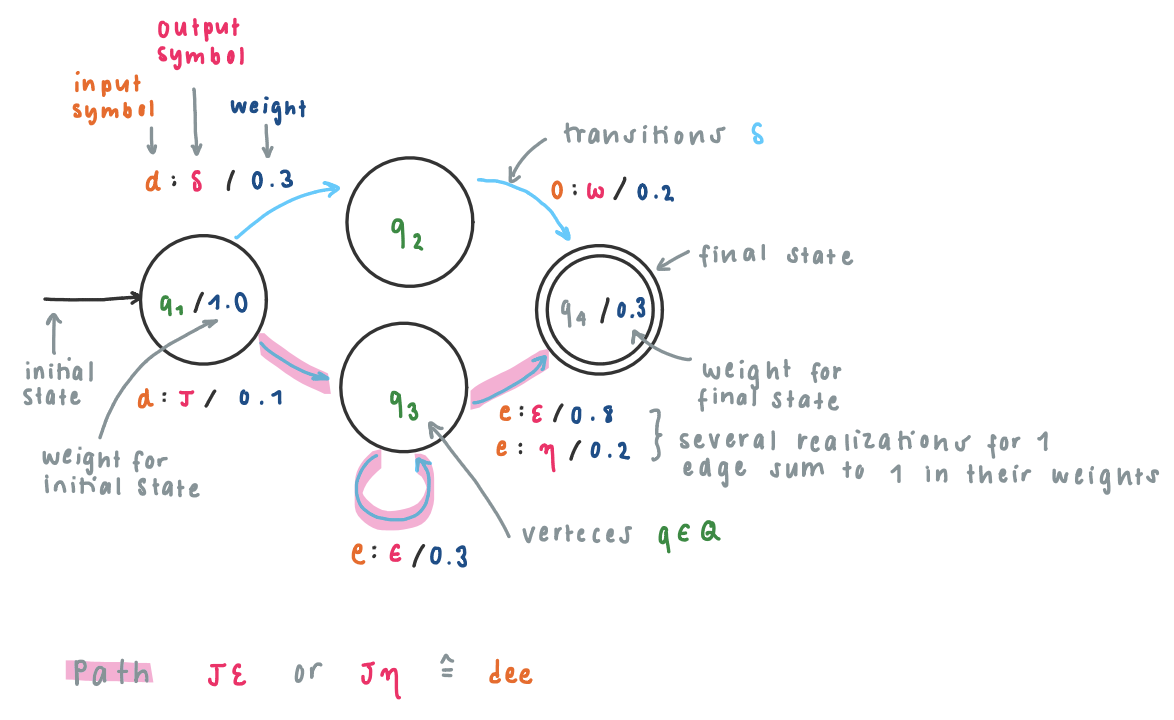
\includegraphics[height=25mm]{inhalt/images/NLP/06_wfsa_1.png}
\\\\
\begin{multicols}{2}
\textit{2) WFST Composition}\\
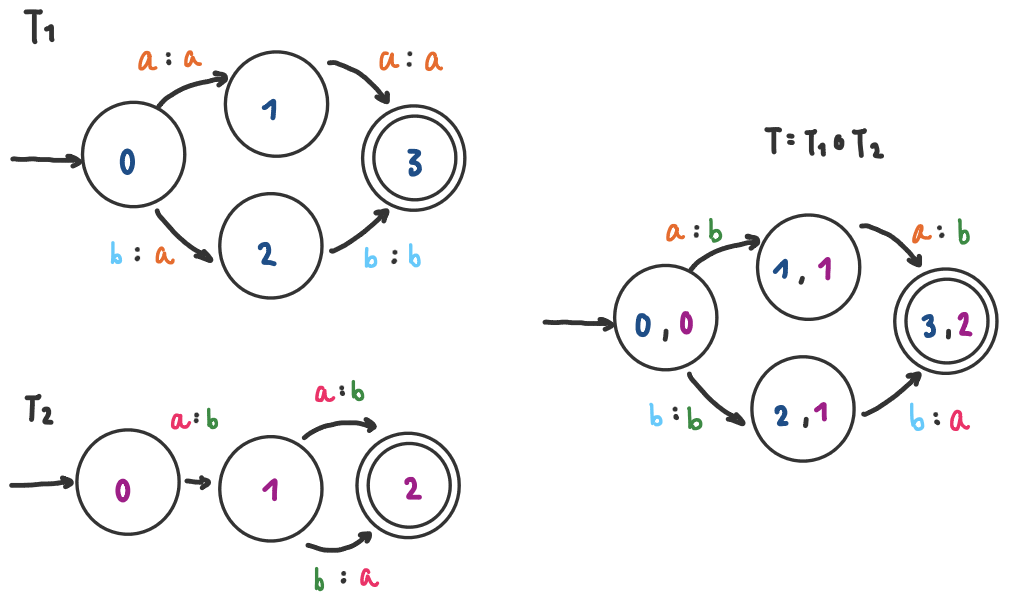
\includegraphics[height=10mm]{inhalt/images/NLP/06_wfsa_2.png}
\\\\
\textit{3) Represent WFSA in matrix form: Adjacency matrix}\\
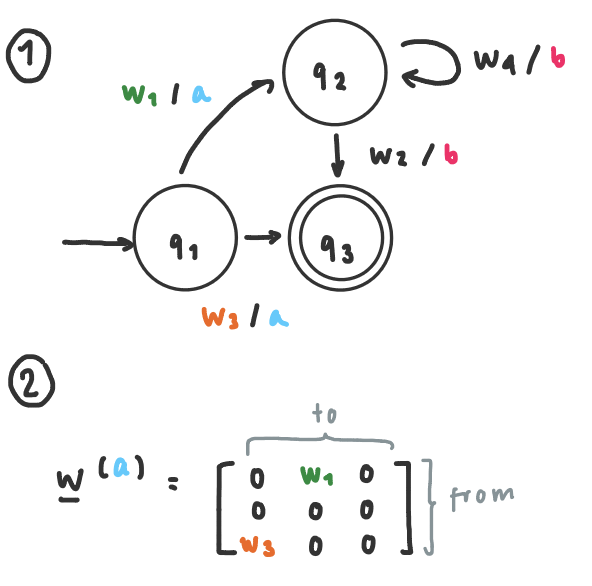
\includegraphics[height=10mm]{inhalt/images/NLP/06_wfsa_3.png}\\\\
\end{multicols}
\textit{4) Lehmann's algorithm: Compute pathsum}\\
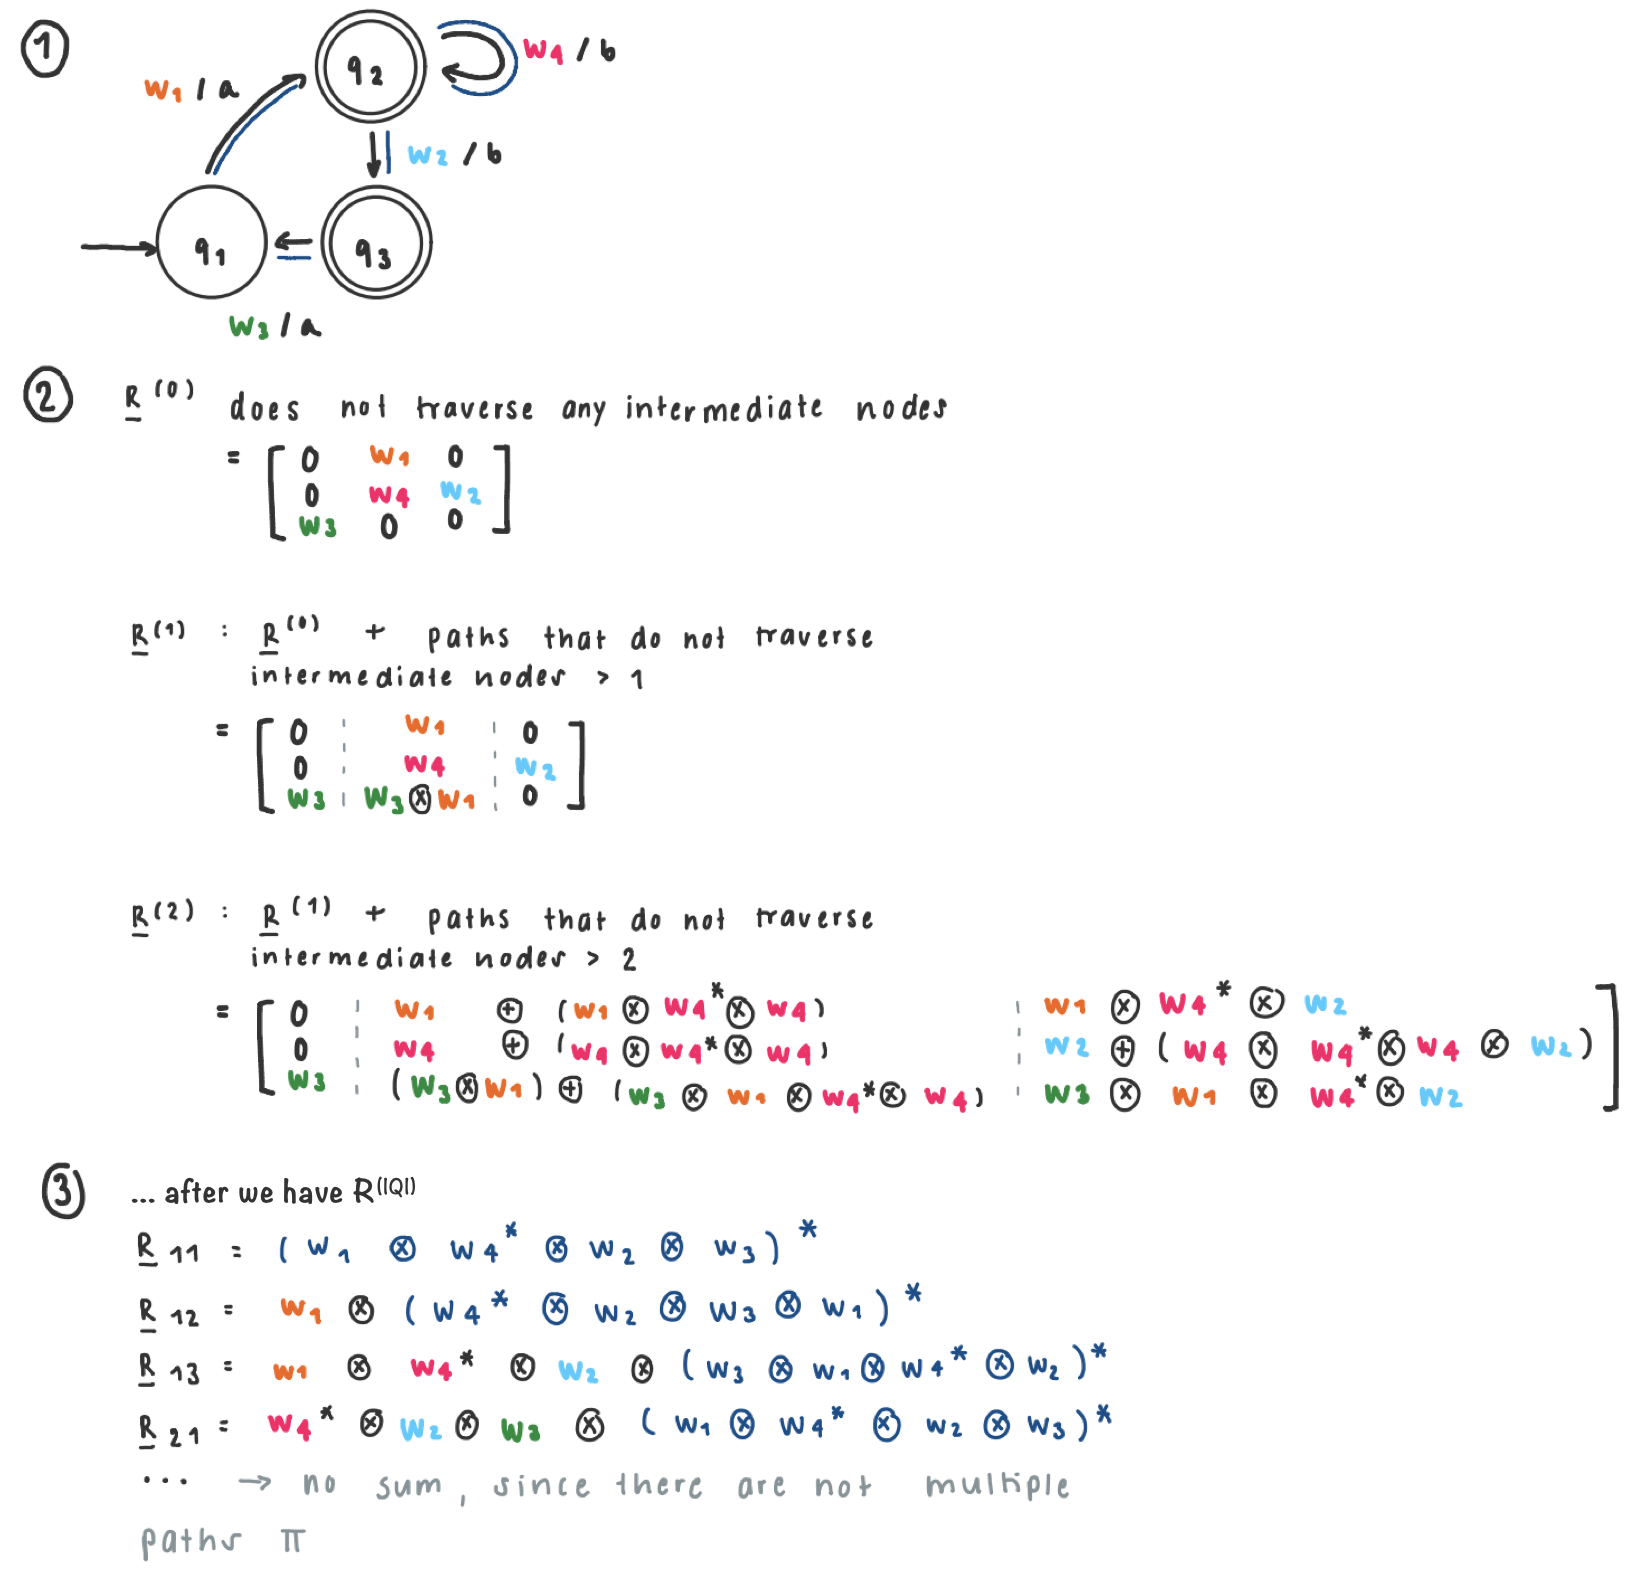
\includegraphics[height=40mm]{inhalt/images/NLP/06_wfsa_4.png}